\section[Empirical Evidence]{Empirical Evidence$^{\text{ JE}}$}
\label{sec:Empirical_evidence}


% {
% \textcite[p. 151 ff]{cookbook} Different Estimation Methods for different setups of the gravity model:




% \begin{itemize}
%     \item Iterative Structural Estimation (+OLS)
%         \item Fixed Effects Estimation (\enquote{Using country fixed effects has an additional advantage that has nothing to do with being consistent with theory.There can be systematic tendencies of a country to export large amounts relative to its GDP and other observed trade determinants. As an example consider the Netherlands and Belgium. Much of Europe’s trade flows through Rotterdam and Antwerp. In principle the production location should be used as the exporting country and the consumption location as the importing country. In practice use of warehouses and other reporting issues makes this difficult so there is reason to expect that trade flows to and from these countries are overstated. Fixed effects can control for this, since they will account for any unobservable that contributes to shift the overall level of exports or imports of a country.})
%         \item Ratio-Type Estimation
%         \item Others (\textcite[p. 154]{cookbook} perform a data generating process to asses different estimation methods via a Monte Carlo Simulation\footnote{Two-Sentence Explanation of Monte Carlo Simulation and why it is important + Source})
% \end{itemize}
% % 
% }







Many gravity based estimation approaches focus solely on international trade in merchandise products. Covering all related findings from that literature alone could fill textbooks. To add value to the discussion of this seminar paper, in section \ref{sec:Goods_Models} we review some interesting findings in regard to trade costs as discussed above and cover results of \textcite[p. 163-166]{cookbook}, who construct a meta-study on 32 scientific papers that estimate trade elasticities with respect to trade costs. Section \ref{sec:Service_Models} then continues to highlight special features of services trade, attempting to provide the reader with a comprehensive overview of this unique field.














% About the PPML est

% The EU-Paper says that this paper proves the consistency of the three way fixed effects method under Poisson estimators, which PPML is.


% “three-way” fixed effects Poisson Pseudo-Maximum Likelihood (“FE-PPML”) estimator with time-varying exporter and importer fixed effects to account for network dependence and time-invariant exporter-importer (“pair” or "group") fixed effects to address endogeneity has recently emerged as a logical workhorse method for empirical trade policy analysis. (\cite{Weidner2021}). Exogenous (in regard to trade flows) IVs for trade policies are especially hard to find when it comes to gravity models, therefore variation along the time dimension can be suitably well used to capture heterogeneous effects of different country pairs. If the assumption of similar trend lines can be empirically assessed and verified, interpretations of causal relationships can be made (\cite{Weidner2021}, \cite{cookbook}). 










\subsection[Results of Goods Trade Applications]{Results of Goods Trade Applications$^{\text{ JE, MK}}$}
\label{sec:Goods_Models}





\textcite{US_Europe} use a combined discrete choice approach with a gravity model to investigate effects of EU domestic market policies on trade outcomes and welfare gains. They apply their model to trade in goods, trade in services and even migration flows as well as capital flows in the form of asset transactions. Using their regression design, they can estimate the costs of cross-border transactions.\begin{figure}[ht]
    \centering
    \caption[Estimates of the Evolution of Trade Costs in Europe: Goods]{Estimates of the Evolution of Trade Costs in Europe: Goods}
    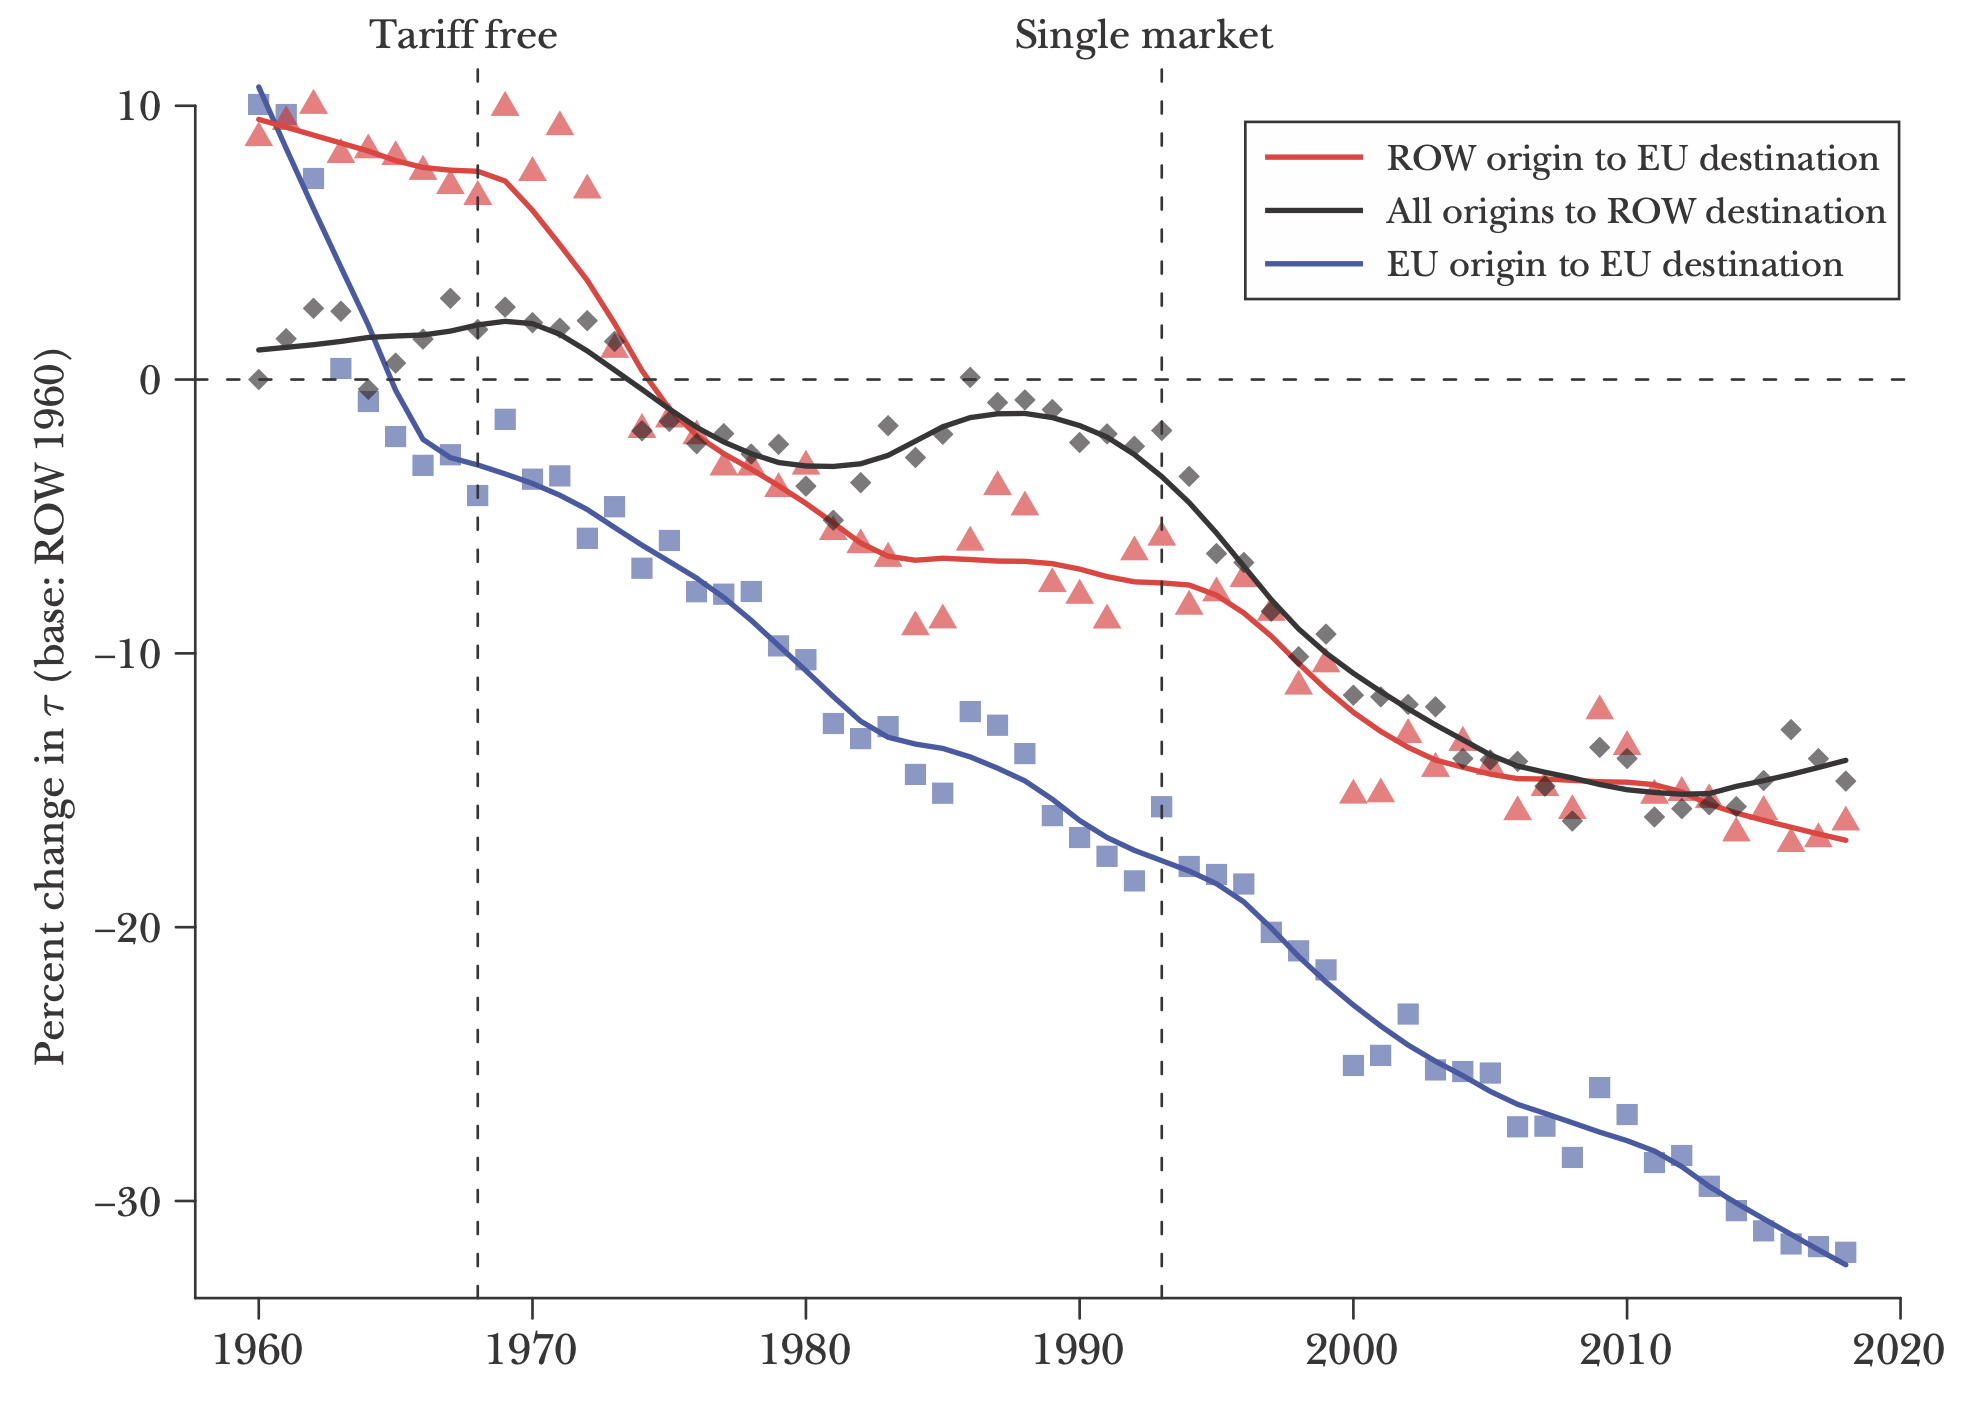
\includegraphics[width=1\textwidth]{IFME/Graphs/Europe_Trade_Costs.png}
    \label{fig:EU_Trade_Costs}
    Figure Source: \cite{US_Europe}\\ Note: \enquote{Each point is obtained by differencing with respect to the 1960 ROW-border coefficient, dividing by $- \epsilon = -5$, exponentiating, subtracting one, and multiplying by 100.} (\cite{US_Europe})
\end{figure} Figure \ref{fig:EU_Trade_Costs} presents the evolution of total trade costs between 1960 and 2018, taking 1960 as a reference year (\cite{US_Europe}). The blue line and squares indicate the change in trade costs between economies that are members of the EU. The red line and triangles illustrate the difference in trade costs compared to the base year for imports from non-EU countries into the EU. The change in trade costs for all trade flows recorded outside the EU is represented by the black line and diamonds. All differences are expressed in percent. The figure shows that in 1960, the costs related to trade to or within the EU were about 10 percent higher, compared to transactions outside the EU. In the subsequent years, a decline in trade costs compared to the base year can be observed, potentially driven in part by the abolishment of tariffs and a closer economic integration between EU member countries. \textcite{US_Europe} state that in 2018, a decrease of trade costs of about 38 percent compared to 1960 can be observed. In contrast, it can be observed that the reduction in trade costs for imports from non-EU members to the EU, as well as trade flows observed outside the EU, showed a less pronounced reduction compared to the base year. However, \textcite{US_Europe} find that trade costs still decreased by about 23 percent compared to 1960 in the case of imports to the EU from outside. 

The above findings indicate that an overall reduction of trade costs has been realised in the past sixty years, regardless of EU membership. However, the effect is more pronounced for trade between EU-countries, supporting the arguments presented in Section \ref{EPF}, that increased economic integration among countries - such as through FTAs, EU-membership, or a common currency - significantly lowers bilateral trade costs. 

































Another discipline that gravity equations can be used for is the estimation of welfare gains from trade liberalization (\cite{old_gains}). A key figure in that regard is the trade cost elasticity of trade as an indicator for the responsiveness of trade flows when costs change. \textcite[p. 163]{cookbook} identify 32 prior papers that estimate such an elasticity by (i) either using a regression framework in which bilateral trade costs (if available) and competitiveness indicators like wage costs, productivity measures or exchange rates are utilized to explain trade flows, or (ii) the elasticity is recovered from ($1-\sigma$) as in equation \ref{eq:bil_trade_costs_SGE} mentioned in section \ref{subsec:estimation_tools}. They provide summary statistics on the trade cost elasticity of trade. These can be seen in table \ref{tab:elasticities_trade_costs}.



\begin{table}[htbp]
    \centering
    \caption[Descriptive Statistics of Price Elasticities in Gravity Equations]{Descriptive Statistics of Price Elasticities in Gravity Equations}
    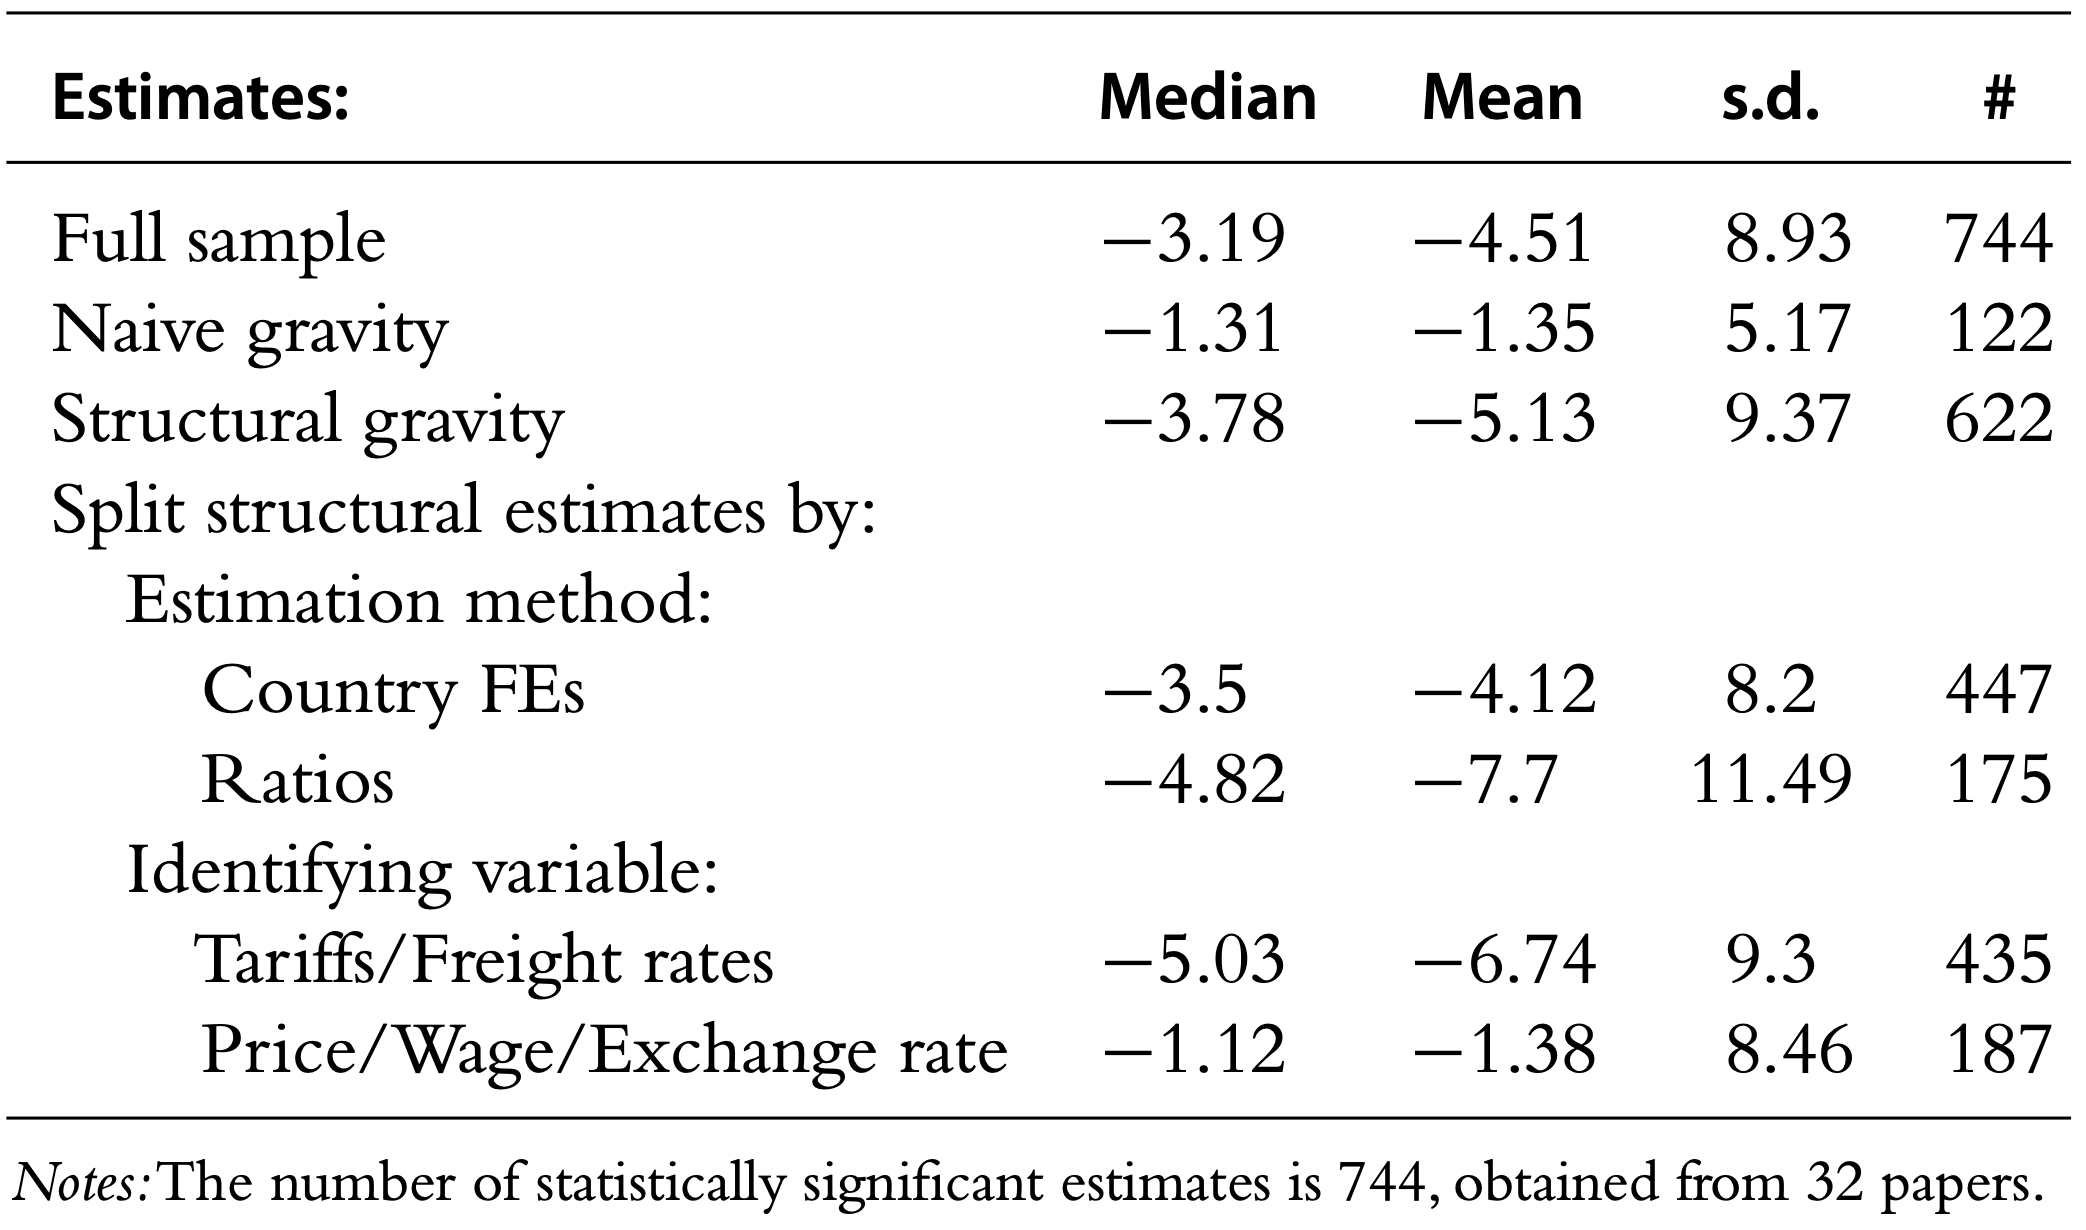
\includegraphics[width=1\textwidth]{IFME/Graphs/elasticities_of_trade_costs.png}
    \label{tab:elasticities_trade_costs}
    Table Source: \cite[p. 164]{cookbook}
\end{table}





Note that the summary statistics were split beginning from the forth row. First, \textcite[p. 164]{cookbook} divide the sample into models that include mutlilateral resistance by either fixed effects or the use of proper ratios, neglecting all studies that have made the \textit{gold medal mistake}. Secondly, only including the filtered studies above, they further split the sample by the covariates included in the regression (see the last two rows of table \ref{tab:elasticities_trade_costs}). The high standard deviation of all the estimates (especially in comparison to the mean) can be traced back to (i) heterogeneity across firms, since many of the papers estimate on the firm level and (ii) the different specifications (\cite[p. 164-165]{cookbook}). Overall, table \ref{tab:elasticities_trade_costs} shows that all mean estimates of trade elasticities with respect to trade costs are larger than one, indicating a general elastic reaction of trade to a change in trade costs. Having an accurate measure of trade elasticities with respect to trade costs is crucial for policy decisions because it determines how significantly trade flows respond to changes in trade barriers, thereby shaping the effectiveness and outcomes of trade liberalization efforts (\cite[p. 165]{cookbook}).





































\subsection[Results of Service Trade Applications]{Results of Service Trade Applications$^{\text{ JE}}$}
\label{sec:Service_Models}


This subsection aims at highlighting the special attributes when it comes to international trade in services and reviews some findings of gravity model applications that quantify effects of trade barriers on cross-border services. Since services are intangible by nature (\cite{intangible_2023}, \cite{eurostat2002manual}), a wide range of classifications into different categories and along different dimensions exists in the literature. A prominent distinction is made by defining the way, in which a service can be supplied across a border. 




\begin{figure}[htbp]
    \centering
    \caption[Synthetic view of modes of service supply]{Synthetic view of modes of service supply set by the \textcite{eurostat2002manual}}
    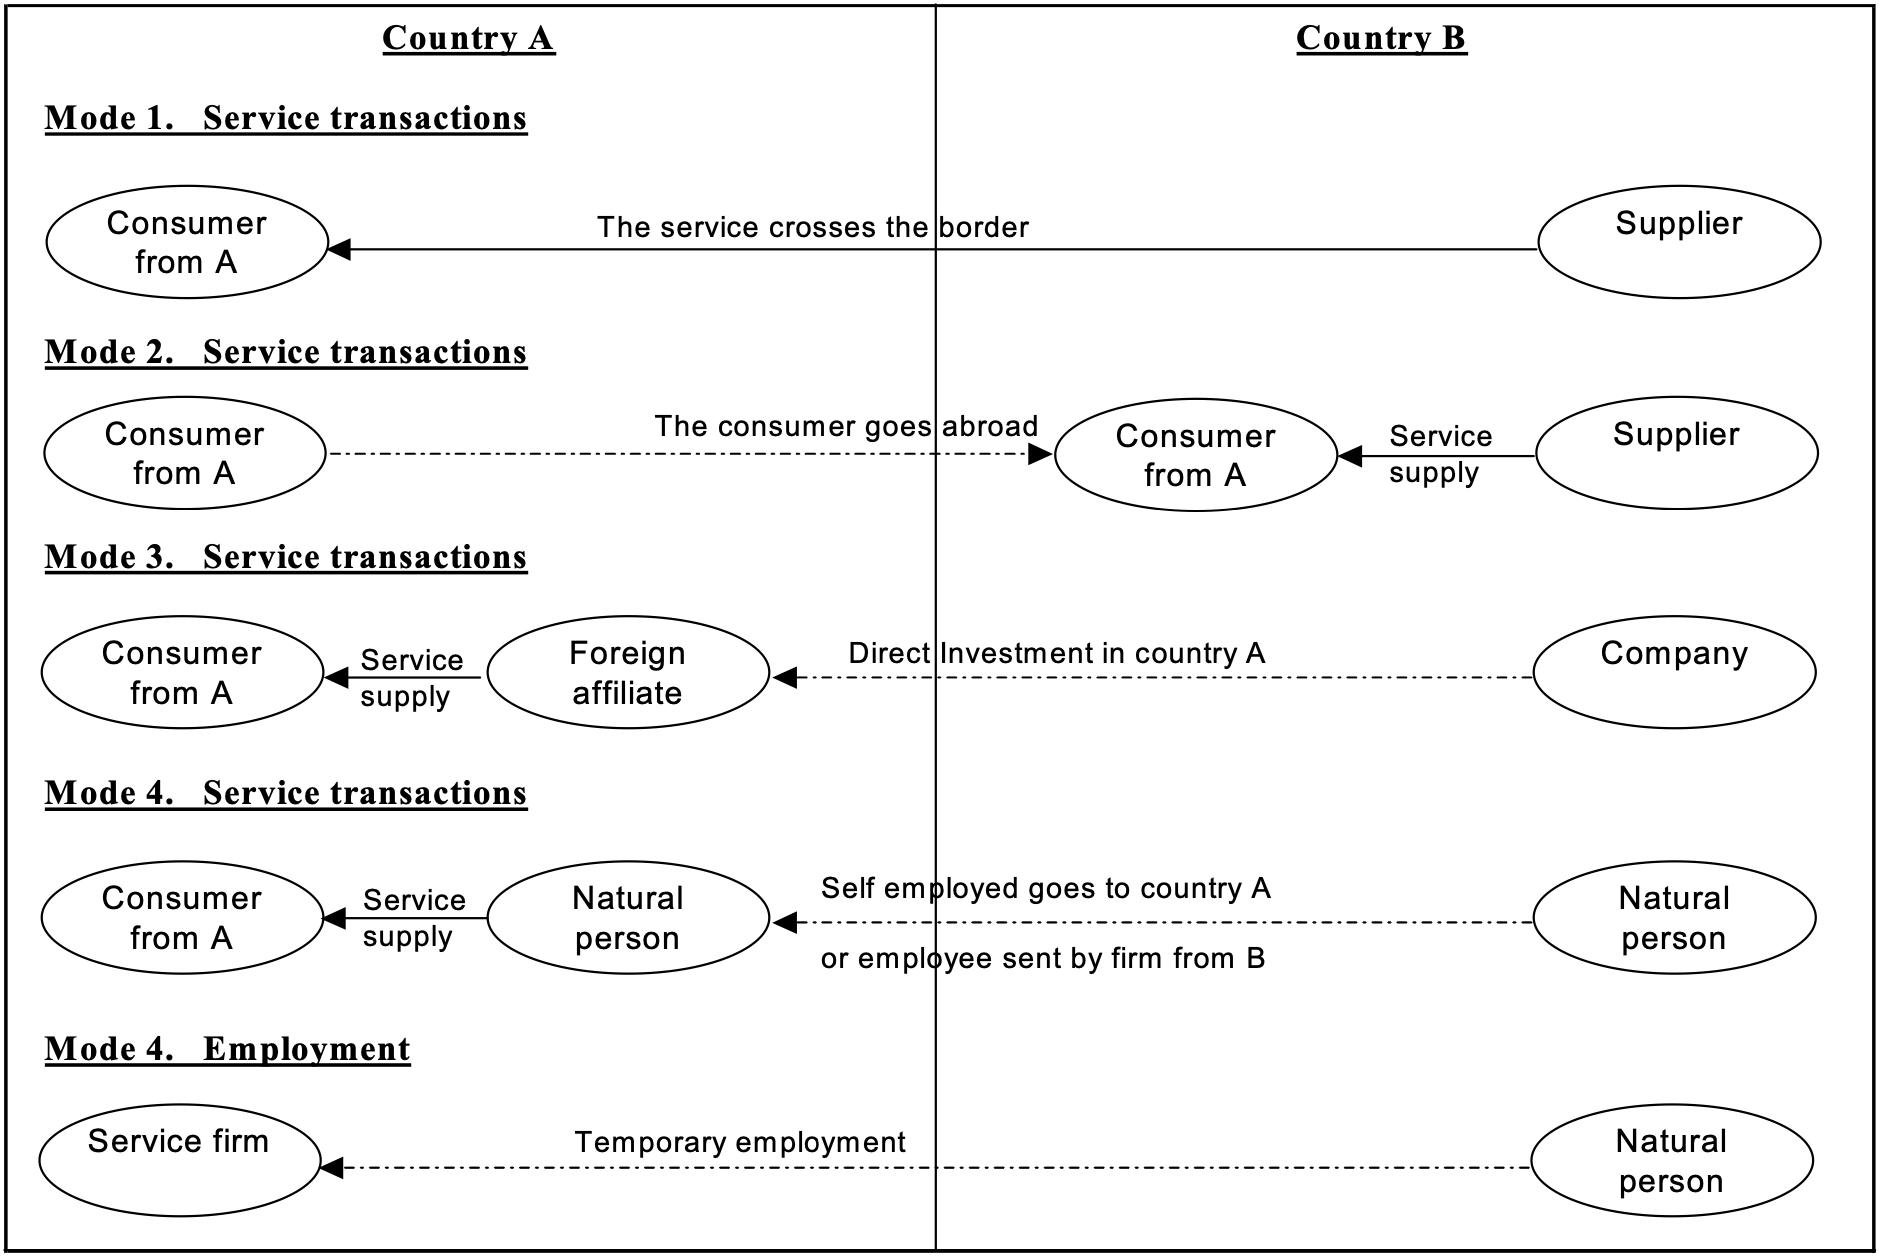
\includegraphics[width=1\textwidth]{IFME/Graphs/Service_supply_modes.png}
    \label{fig:service_modes}
    \small 
    Figure Source: \cite[p. 25]{eurostat2002manual}
\end{figure}



The four modes that supply of services trade (from here called \textit{mode x}) could take are defined in the General Agreement on Trade in Services (GATS). Broadly, \textit{mode 1} can be summarized as the cross-border supply of services, \textit{mode 2} represents service consumption abroad, \textit{mode 3} stands for the commercial presence of foreign service companies and finally, \textit{mode 4} includes all cross-border movements of natural persons. Figure \ref{fig:service_modes} illustrates these modes and provides intuition of real world applications.









\textcite{Breinlich_and} also highlight the relatively higher importance of heterogeneity across firms when it comes to trade in services compared to trade in goods. They mainly provide a classification of three important classes of services when it comes to international trade: (i) producer services (inputs in production of other services and goods), (ii) services that involve travel of persons and (iii) transportation services. Along these classes they identify differences in (i) the number of foreign markets served, (ii) the value of exports and imports per served market and (iii) the share of individual markets in overall sales. 

To present stylized facts about trade in services \textcite{Breinlich_and} assess how well heterogeneous firms gravity models from the literature can be utilized to construct analysis in service sectors. They find that a large amount of the existing covariates (language dummy, border dummy, colonial ties and so on) are also determinants for trade in services and therefore, such models are implied to be a starting point for further empirical studies.\footnote{This is inline with findings of \textcite{Walsh2006}, who also points out that the gravity equation can be used well to asses determinants of services trade, once empirical estimation tools overcome sources of bias, like firm heterogeneity.} Merging the Annual Respondents Database for the UK and the International Trade in Services Inquiry, \textcite{Breinlich_and} produce a rather disaggregated dataset to determine the extensive margin (number of traders and service types per country) and intensive margin (average trade per firm and service type) an thus, explain micro patterns of services trade. They also indirectly imply that trade barriers for services differ in their nature from barriers for goods. 




Generally, the assessment and estimation of trade barriers in services trade is more complex than in goods trade and therefore, harder to quantify in an empirical setup. Trade barriers in services trade often take the form of legal or institutional regulations, instead of tariffs or other \textit{easily} quantifiable barriers when it comes to goods trade (\cite{Trade_Barriers_Korea}). Imposing tariffs or restricting services through import quotas turns out to be difficult for a service when referring to the original definition, in which the supply and consumption of a service occurs simultaneously (\cite{Trade_Barriers_Korea}). Therefore, regulations that classify as trade barriers in services are usually laid upon the providing firms themselves. Broadly, \textcite{Trade_Barriers_Korea} summarize examples for such service trade barriers as (i) obtaining licenses (induced with cross-border restrictions), (ii) environmental regulations and standards, (iii) acceptance and refusal of certificates and academic degrees, (iv) government service demand policies that favor domestic providers and finally, (v) exporting service firms often need to utilize foreign distribution networks or existing infrastructure. Any regulation that systematically discriminates foreign service providers from using these networks compared to domestic ones can also be classified as a service trade barrier. \textcite{Trade_Barriers_Korea} continue to first estimate the structural gravity model (without the inclusion of mutlilateral resistance terms) excluding trade barriers in the model. The fitted values of that model are then used to forecast trade flows. These forecasts are than compared to actually observed data. \textcite{Trade_Barriers_Korea} use the observed differences backwards to proxy trade barriers with the focus on business, financial and transportation services due to limited data availability. Their main result is the estimation of tariff equivalents for different countries that describes in percentage (relative to a benchmark country with the lowest estimated trade barriers) how strong trade barriers in services are. 







\textcite{intangible_2023} investigate sector heterogeneity when it comes traded services and give more detailed insights into different trade barriers for different industries. They provide a rich class categories to describe different aspects in this field. First, they split the underlying characteristics among different service industries into the three dimensions (i) \textit{the level of customer interaction needed}, (ii) \textit{the level of online marketability} and \textit{the level of skill required to supply the service}. Using the modes of service supply as discussed above and shown in figure \ref{fig:service_modes}, \textcite{intangible_2023} apply the idea of these dimensions to the different industries and argue that some sectors might utilize all four modes (e.g. legal services), while others predominantly supply through one mode (e.g. travel and tourism, as this mainly involves mode 2). They continue by considering 13 different service sectors and place them into three parent categories: (i) \textit{data-intensive services}\footnote{As \textit{data-intensive services} \textcite{intangible_2023} list \enquote{telecommunications, computer, and insurance services}.}, (ii) \textit{transportation and related services}\footnote{As \textit{transportation and related services} \textcite{intangible_2023} list \enquote{air transport, road, rail, and sea freight transport, logistics, and postal and courier services}.} and (iii) \textit{professional and related services}\footnote{As \textit{professional and related services} \textcite{intangible_2023} list \enquote{legal, accounting, architecture and engineering, and construction services}.}. Furthermore, \textcite{intangible_2023} proceed by analyzing the sub-sectors of these broader categories through the decomposition of the STRI along the four modes of supply from figure \ref{fig:service_modes}.


\begin{figure}[ht]
    \centering
    \caption[Average STRI scores by mode of supply, 2014-2017.]{Average STRI scores by mode of supply, 2014-2017.}
    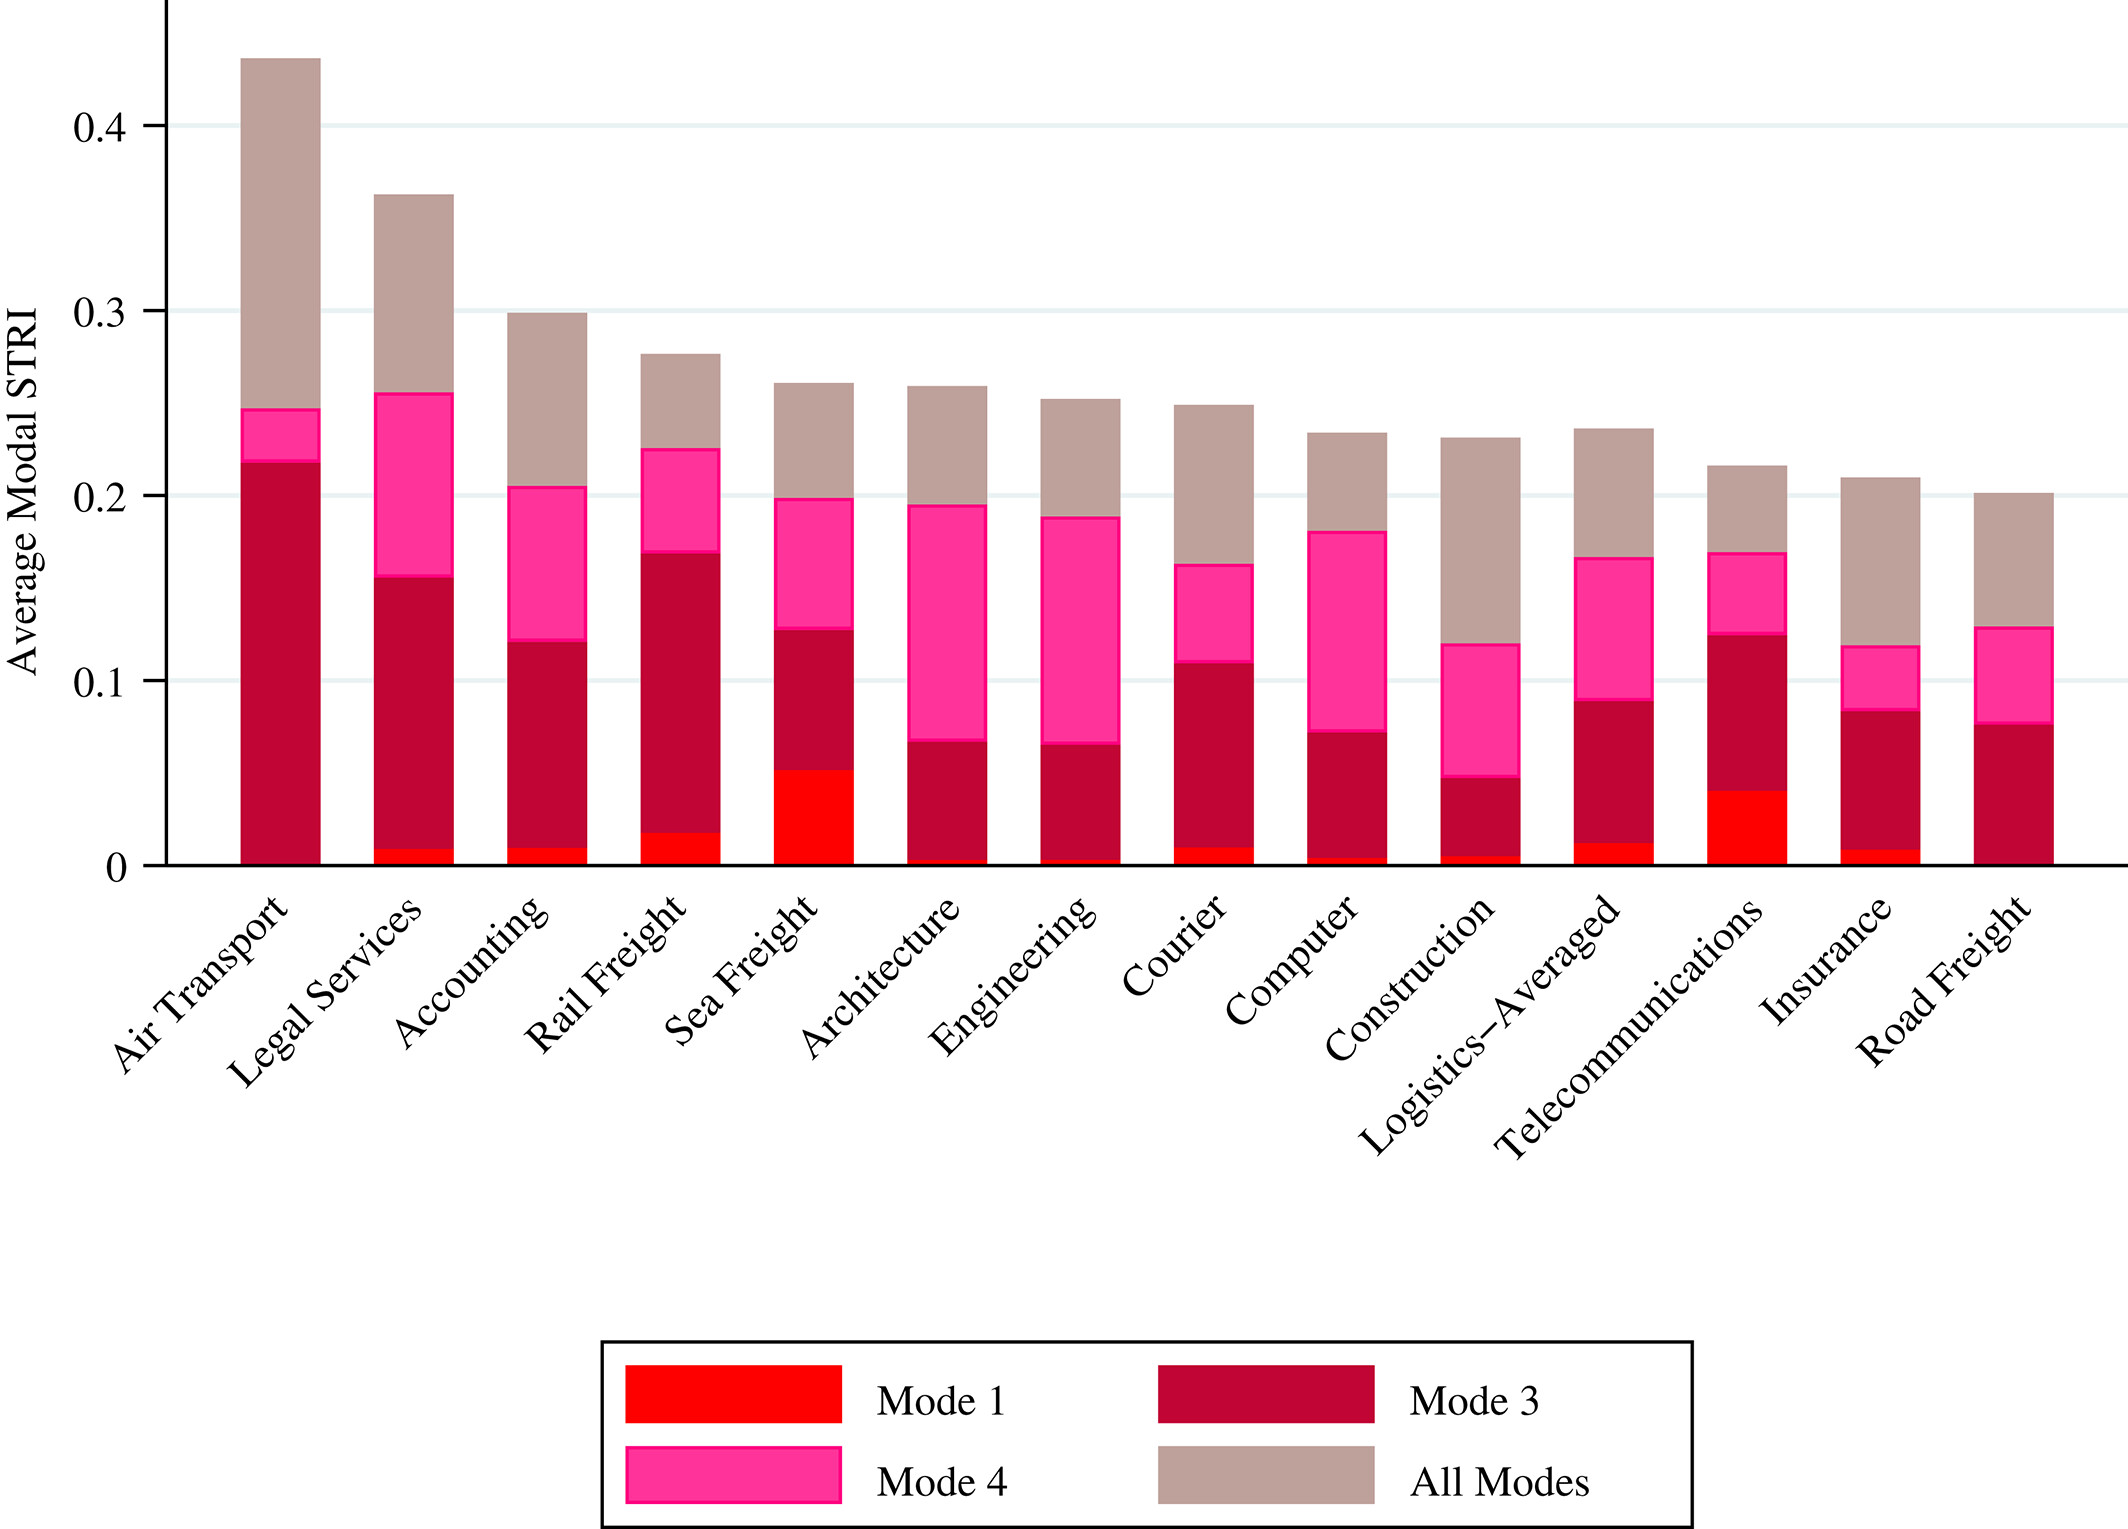
\includegraphics[width=1\textwidth]{IFME/Graphs/STRI_mode.jpeg}
    \label{fig:STRI_modes}
    \small 
    \enquote{Modal STRI values averaged over the years and observations in the data sample.} \\
    Figure Source: \cite{intangible_2023} \\ Online Link: \href{https://onlinelibrary.wiley.com/doi/10.1111/twec.13346  }{wileyonlinelibrary.com}
\end{figure}



Figure \ref{fig:STRI_modes} shows how the reviewed industries' STRI\footnote{Logistics sector is excluded.} looks disaggregated across the modes of supply. Note that mode two is not included, since mode two is characterized by the mobility of the customer (see figure \ref{fig:service_modes}). Therefore, any trade barriers that are relevant for that mode mainly depend on bilateral regulations (e.g. visa requirements) and must not be distinguished on the sector level (\cite{intangible_2023}). Mainly, figure \ref{fig:STRI_modes} provides insights which types of regulations that act as service trade barriers are important for which industries, and to what extent. For instance, computer services can be seen to be effected very little by mode one barriers like data flow restrictions, while mode four barriers - like temporary entry limits of natural persons - restrict computer services trade relatively strong. The authors find adequate words to explain this: \enquote{While many of the activities that fall under computer services, such as electronic delivery of software, do not require physical presence to export, other services, such as cloud infrastructure, tend to benefit from local infrastructure to improve customer experience.} (\cite{intangible_2023}). Figure \ref{fig:STRI_modes} also shows that air transport services are, on average, the most restricted in the selected sample, mainly by regulations that effect all supply modes and specifically mode 3 policies such as foreign equity participation or public ownership (\cite{intangible_2023}). Disaggregating these trade barriers subject to the shown industries sheds light on the often unobserved heterogeneity in services trade by sectors. Another example is the telecommunications industry, for which mode three barriers make up relatively most of the overall STRI. \textcite{intangible_2023} point out that antitrust regulations on \enquote{[…] cross-border mergers and acquisitions, foreign branch limits and data flow restrictions} can be seen as the most important ones for this sector.\footnote{To find further insights on specific policies that hamper trade in the respective industries, see \textcite{intangible_2023}.} 

The main value \textcite{intangible_2023} then add to the literature is by using the structural gravity model to investigate the relationship of mode three barriers (e.g. limitations on foreign equity shares) to traded services in all other modes. Contrary to findings before, they conclude that mode three trade acts complementary to the other modes, instead of having a substitutable nature. The intuition is as follows. If mode three trade and the rest of the modes are assumed to be substitutes, a policy that would reduce mode three trade - like restrictions on foreign direct investments (FDI) in foreign affiliates - would lead to a rise in services trade in the other modes. In that case it is implied that welfare reductions due to less trade in mode three are compensated to some extent by the achieved trade gains from the other modes. The opposite would be the case if a complementary relationship is assumed. A regulation aimed at reducing FDI would lead to less exports in mode 3 services as well as the other modes. In combination with their finding of a complementary relationship, \textcite{intangible_2023} therefore conclude that policies to liberalize mode three trade can positively effect welfare through gains from trade in all service modes.

In addition to this, \textcite{trade_agreements_2024} explore the impact of trade agreements on services trade, providing a differentiated analysis of different types of agreements, particularly General Trade Agreements (GTAs) and Deep Trade Agreements (DTAs). While tariff reductions through RTAs are found to boost trade in goods strongly, their effect on services trade is smaller (\cite{trade_agreements_2024}). Their primary contribution lies in examining the heterogeneous effects of these agreements, noting that higher institutional quality in high-income countries leads to stronger service market integration. \textcite{trade_agreements_2024} highlight the effectiveness of DTAs by addressing behind-the-border barriers, thereby lowering service trade costs and improving the business environment. They use the PPML estimator within a difference-in-differences framework to be able to also make causal conclusions.\footnote{\textcite{trade_agreements_2024} also provide robustness checks to mitigate potential endogeneity concerns and use propensity score matching to address the self-selection bias of RTAs.}









To highlight the wide range of possible applications of the gravity framework, we want to mention two more aspects that help to better understand the complex nature of services trade. First, \textcite{religion} shows that religion can also be viewed as a determinant of trade and effects international trade through two channels. The first one are network effects that can be generated by enhancing trust between trading partners that share the same religious beliefs and thus, bilateral distance in the sense of transaction costs can be reduced. Secondly, heterogeneous institutional effects take place, i.e. some religious regimes promote openness and trade, whereas others hamper it.\footnote{\textcite{religion} does also not analyse the extant of heterogeneity relating to the institutional effects of religion on trade. Their implications can only be interpreted at the aggregate level.} Overall, \textcite{religion} uses a gravity based PPML estimation approach without incorporation of multilateral resistance terms (thus, committing the gold medal mistake)\footnote{Therefore, the implications have to be considered with great care.} to find that a common religion fosters trade through these two channels. Interestingly, \textcite{religion} also run their model both on trade in goods and trade in services and show that the impact of religion is larger in services sectors than in goods sectors. This finding highlights again the nature of services trade, in which suppliers and consumers have to engage in a more close relationship than, for instance, a firm that exports merchandise to its customers.  



Finally, the above mentioned network effects and interdependencies are of special importance and become more frequently addressed in recent literature. As pointed out by \textcite{understanding_2023}, the inclusion of proper mutlilateral resistance terms reflect to some extent such network interdependencies, however, only on the surface level. In reality, global value chains become more complex and intermediate inputs in the production of goods and services are increasingly characterized by non-physical attributes (\cite{understanding_2023}). Especially digital services as intermediate inputs in global value chains develop quickly and are complex in nature. \textcite{understanding_2023} therefore utilize a social network approach, accounting for the \textit{connectivity} of trading partners with their respective trading partners' partners. They use this method to create network interdependency indicators which they then include in a two-stage gravity model approach, where the first stage is computed using the PPML estimator and the second stage, including the constructed indicators, is estimated using OLS.\footnote{\textcite{understanding_2023} carefully examine the inclusion of fixed effects as well as multilateral resistance terms in their two-stage estimation process and reflect on potential sources of bias.} Their findings indicate that the cross-border digital services embodied in gross exports build an even more heterogeneous value chain network than that of the general global trade. Moreover, \textcite{understanding_2023} point out that market access costs of firms engaged in cross-border digital services can be substantially lowered by having a strengthened network, including well connected trading partners. The intuition is that knowledge spill-overs of partner firms can ease the entrance of new foreign markets by implicitly lowering service trade barriers (\cite{understanding_2023}). As digital services rapidly evolve and technological progress might face a new era of growth due to new discoveries in the field of convolutional neuronal networks and artificial intelligence, ongoing research on the heterogeneous nature and complexity of global digital service networks will be needed to understand future trade dynamics.











